\documentclass[a4paper, fleqn]{scrartcl}

\usepackage[ngerman]{babel}
\usepackage[utf8]{inputenc}
\usepackage{amsmath}
\usepackage[T1]{fontenc}
\usepackage{lmodern}
\usepackage{graphicx}
\usepackage{tikz}

\title{Übung - Paketübertragung}
\author{Fabian Wolter, Selin Kabak}
\date{}

\begin{document}
\maketitle
%\tableofcontents

\section{Ende-zu-Ende-Verzögerung}
\begin{tabular}{l|l|l|l}
      & Übertragungsrate & Physikalische Länge & Physikalische Ausbreitungsgeschwindigkeit \\
      \hline
      Link 1 & 60 Mbit/s & 15 m & 300000 km/s \\
      Link 2 & 25 Mbit/s & 250 m & 200000 km/s \\
      Link 3 & 20 Gbit/s & 10 km & 250000 km/s
\end{tabular}
\subsection{Bestimmen Sie die Ausbreitungsverzögerung und die Übertragungsverzögerung der drei Links für Pakete der Größe 1500 Byte.}
\[\text{Ausbreitungsverzögerung}=\frac{\text{Physikalische Länge}}{Ausbreitungsgeschwindigkeit}\]
\[\text{Übertragungsverzögerung}=\frac{\text{Paketgröße}}{\text{Übertragungsrate}}\]
Link1:\\
\[\text{Ausbreitungsverzögerung}=\frac{0,015km}{300000km/s}=0,00000005s=0,00005ms\]
\[\text{Übertragungsverzögerung}=\frac{12000bits}{60Mbit/s}=0,0002s=0,2ms\]
Link2:\\
\[\text{Ausbreitungsverzögerung}=\frac{0,25km}{200000km/s}=0,00000125s=0,00125ms\]
\[\text{Übertragungsverzögerung}=\frac{12000bits}{25Mbit/s}=0,00048s=0,48ms\]
Link3:\\
\[\text{Ausbreitungsverzögerung}=\frac{10km}{250000km/s}=0,00004s=0,04ms\]
\[\text{Übertragungsverzögerung}=\frac{12000bits}{20Gbit/s}=0,0000006s=0,0006ms\]
\subsection{Bestimmen Sie die Ende-zu-Ende-Verzögerung für die Übertragung eines Pakets über die drei Links in der Reihenfolge 1-2-3. Hängt die Ende-zu-Ende-Verzögerung von der Reihenfolge der Links ab?}
\[\text{Verzögerung}=0,00005ms+0,2ms+0,00125ms+0,48ms+0,04ms+0,0006ms=0,7219ms\]
Die Reihenfolge der Links hat keinen Einfluss auf die Ende-zu-Ende-Verzögerung, da die Verzögerungen der Links addiert werden.
\subsection{Betrachten Sie nun einen Paket-Burst aus 20 Paketen, d.h. 20 Pakete werden direkt hintereinander übertragen werden. Was ist die Gesamtübertragungsdauer für diesen Paketburst, wenn die Links in der Reihenfolge 1-2-3 verwendet werden? Hängt die Gesamtübertragungsdauer von der Reihenfolge der Links ab?}
\[\text{Gesamtübertragungsdauer}=1\cdot0.7219ms+19\cdot0,48ms=9,8419ms\]
Bei den 20 Paketen wird nur beim ersten Paket die Ausbreitungsverzögerung addiert, bei den restlichen Paketen nur die Übertragungsverzögerung, da die Pakete direkt hintereinander übertragen werden und somit ein Pipelining stattfindet.
Die Reihenfolge der Links hat keinen Einfluss auf die Gesamtübertragungsdauer, da die Verzögerungen der Links addiert werden.

\section{Durchsatz und Paketverlust}
Gegeben sei die in Abbildung 1 dargestellte Übertragungsstrecke von einer Quelle $Q$ zu einem Ziel $Z$, die über vier Router $R_1$ bis $R_4$ verläuft.
Die Link-Kapazitäten sowie die Ausbreitungsverzögerungen der fünf Links sind in der Abbildung angegeben. Jedes Paket enthält 600 Bytes.
\begin{figure}[h]
\centering
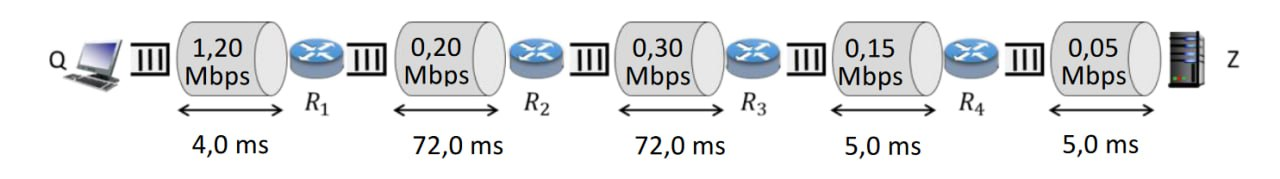
\includegraphics[width=\textwidth]{übertragunsstrecke.png}
\caption{Übertragungsstrecke}
\end{figure}
\subsection{Bestimmen Sie die Ende-zu-Ende Übertragungsdauer für ein Paket.}
Paket in Bits: $600B\cdot8\frac{b}{B}=4800b$\\
\begin{itemize}
    \item Link 1: $\frac{4800bits}{1,20\cdot10^6bits/s}=0,004s=4ms$\\
    \item Link 2: $\frac{4800bits}{0,20\cdot10^6bits/s}=0,024s=24ms$\\
    \item Link 3: $\frac{4800bits}{0,30\cdot10^6bits/s}=0,016s=16ms$\\
    \item Link 4: $\frac{4800bits}{0,15\cdot10^6bits/s}=0,032s=32ms$\\
    \item Link 5: $\frac{4800bits}{0,05\cdot10^6bits/s}=0,096s=96ms$\\
\end{itemize}
Ende-zu-Ende Übertragungsdauer:\\ $4ms+24ms+16ms+32ms+96ms+4ms+72ms+72ms+5ms+5ms=330ms$

\subsection{Die Quelle $Q$ versendet Pakete mit einem Abstand von 8,00 ms}
\subsubsection{Bestimmen Sie für jeden Link den prozedualen Anteil der Angekommenen Pakete, die langfristig verloren gehen.}
\begin{itemize}
    \item Link 1: $0\%$
    \item Link 2: $1-\frac{8ms}{24ms}=66,67\%$
    \item Link 3: $1-\frac{8ms}{16ms}=50\%$
    \item Link 4: $1-\frac{8ms}{32ms}=75\%$
    \item Link 5: $1-\frac{8ms}{96ms}=91,67\%$
\end{itemize}
\subsubsection{Bestimmen Sie die physikalische Länge und die Anzahl gleichzeitiger Pakete für den Link zwischen $R_1$ und $R_2$, wenn die Ausbreitungsgeschwindigkeit 200000 km/s beträgt.}
\begin{align*}
    \text{Distanz} &= \text{Ausbreitungsgeschwindigkeit}\cdot\text{Ausbreitungsverzögerung}\\
    &= 200000km/s\cdot0,072s=14,400km\\
    \text{Maximale Anzahl Bits} &= \text{Übertragungsrate}\cdot\text{Ausbreitungsverzögerung}\\
    &= 0,20Mbit/s\cdot0,072s=0,0144Mbit=14,4kbit\\
    \text{Anzahl der Pakete} &= \frac{14,4kbit}{4800bit}=3
\end{align*}
\subsection{Skizzieren Sie die physikalische Ausdehnung der Pakete (physikalische Länge und Abstand) für die Links zwischen $R_1$ und $R_2$ sowie zwischen $R_2$ und $R_3$. Die Linie entspricht der physikalischen Länge der Links}
Link $R_1$ zu $R_2$:
\begin{tikzpicture}
    \draw[line width=1em] (0,0) -- (2.9,0);
    \draw[line width=1em] (3,0) -- (5.9,0);
    \draw[line width=1em] (6,0) -- (8.9,0);
\end{tikzpicture}
\\
Link $R_2$ zu $R_3$:
\begin{tikzpicture}
    \draw[line width=1em] (0,0) -- (1.9,0);
    \draw[line width=1em] (3,0) -- (4.9,0);
    \draw[line width=1em] (6,0) -- (7.9,0);
\end{tikzpicture}
\subsection{Die Quelle $Q$ versendet Pakete zu den folgenden Zeitpunkten: 0,0 ms (900 B); 2,0 ms (600 B); 3,0 ms (900 B); 4,0 ms (900 B); 5,0 ms (900 B); 7,0 ms (1200 B); 9,0 ms (900 B); 24 ms (1200 B); 26 ms (1200 B); 27 ms (1200 B). Bestimmen Sie mit Hilfe einer Ereignistabelle, welche Pakete zwischen Quelle $Q$ und Router $R_1$ verloren gehen, wenn der Aufgangs-Puffer von $Q$ zu $R_1$ drei Pakete aufnehmen kann.}
\begin{tabular}{|l|l|l|l|l|}
    \hline
    Paket & Ankunftszeit (ms) & Größe (B) & Größe (b) & Übertragungszeit (ms)\\
    \hline
    1 & 0,0 & 900 & 7200 & 6\\
    2 & 2,0 & 600 & 4800 & 4\\
    3 & 3,0 & 900 & 7200 & 6\\
    4 & 4,0 & 900 & 7200 & 6\\
    5 & 5,0 & 900 & 7200 & 6\\
    6 & 7,0 & 1200 & 9600 & 8\\
    7 & 9,0 & 900 & 7200 & 6\\
    8 & 24,0 & 1200 & 9600 & 8\\
    9 & 26,0 & 1200 & 9600 & 8\\
    10 & 27,0 & 1200 & 9600 & 8\\
    \hline
\end{tabular}
\newline
\vspace{1em}
\newline
\begin{tabular}{|l|l|l|l|}
    \hline
    Zeit (ms) & Ereignis & Anzahl Pakete im Puffer & Ende der\\
    & & & Übertragung (ms)\\
    \hline
    0,0 & 1 kommt an & 1 & 6,0\\
    2,0 & 2 kommt an & 2 & 10,0\\
    3,0 & 3 kommt an & 3 & 16,0\\
    4,0 & 4 kommt an (dropped) & 3 & --\\
    5,0 & 5 kommt an (dropped) & 3 & --\\
    6,0 & 1 wird übertragen & 2 & --\\
    7,0 & 6 kommt an & 3 & 24,0\\
    9,0 & 7 kommt an (dropped) & 3 & --\\
    10,0 & 2 wird übertragen & 2 & --\\
    16,0 & 3 wird übertragen & 1 & --\\
    24,0 & 8 kommt an & 2 & 32,0\\
    24,0 & 6 wird übertragen & 1 & --\\
    26,0 & 9 kommt an & 2 & 34,0\\
    27,0 & 10 kommt an & 3 & 42,0\\
    32,0 & 8 wird übertragen & 2 & --\\
    34,0 & 9 wird übertragen & 1 & --\\
    42,0 & 10 wird übertragen & 0 & --\\
    \hline
\end{tabular}

\end{document}